
%(BEGIN_QUESTION)
% Copyright 2014, Tony R. Kuphaldt, released under the Creative Commons Attribution License (v 1.0)
% This means you may do almost anything with this work of mine, so long as you give me proper credit

An interesting chemical analyzer mechanism used by German chemical manufacturers near the time of World War II used a four-element Wheatstone bridge circuit where each element was a platinum wire heated by the bridge's excitation current, changing temperature as a function of convective gas cooling.  The greater the cooling effect of the gas, the lower the wire temperature and therefore the less electrical resistance each wire sensor exhibited:

$$\includegraphics[width=15.5cm]{i00979x01.eps}$$

Manually-adjusted restrictor valves were set by instrument technicians to maintain equal flow rates of each gas stream (as measured at the vents).

\vskip 10pt

Given that hydrogen gas has a much greater specific heat than carbon dioxide gas, identify the polarity of voltage signal across the voltmeter as the carbon dioxide concentration becomes stronger.

\vskip 20pt \vbox{\hrule \hbox{\strut \vrule{} {\bf Suggestions for Socratic discussion} \vrule} \hrule}

\begin{itemize}
\item{} A good problem-solving technique to apply in cases where we need to determine the direction of a change is to consider {\it limiting cases}.  Instead of asking ourselves what would happen if the CO$_{2}$ concentration changed slightly, we ask ourselves what would happen if the CO$_{2}$ concentration changed {\it dramatically}.  Explain how this problem-solving technique applies to this particular system.
\item{} What assumption(s), if any, must we make about the sample gas in order to trust the readings given by this analyzer?
\item{} Identify the purpose of the three-way valve shown in the diagram.
\item{} Which way should the ``span adjustment'' potentiometer wiper be moved to make this instrument more sensitive (i.e. generate a greater voltage at the voltmeter for any given concentration of CO$_{2}$ in the sample gas).
\end{itemize}

\underbar{file i00979}
%(END_QUESTION)





%(BEGIN_ANSWER)

If there is no CO$_{2}$ in the sample gas at all, all four resistance cells will experience the exact same amount of cooling, and the bridge will be balanced.

\vskip 10pt

As sample gas CO$_{2}$ concentration increases, the relative concentration of hydrogen increases in the green-colored tubing compared to the red-colored tubing because the CO$_{2}$ is being absorbed by the potassium hydroxide (KOH) solution.  Since hydrogen has a much greater specific heat than carbon dioxide, the pure hydrogen (green) stream will have greater cooling capacity than the mixed (red) stream, causing the green-shaded resistance cells to decrease in resistance.  This unbalances the bridge, making the left-hand terminal of the voltmeter negative and the right-hand terminal positive.

%(END_ANSWER)





%(BEGIN_NOTES)

An interesting feature of this analyzer is a colorimetric indicator technicians would add to the 25\% KOH solution to indicate when it needed to be refreshed.  To each liter of 25\% KOH solution, one cm$^{3}$ of ``indicator'' solution was added, comprised of 4 grams thymolphthalein dissolved in 90\% pure alcohol.  The normal color of this indicator (in strong KOH) was blue.  As the KOH solution grew weaker due to acidification from the CO$_{2}$ gas, the solution became colorless.

\vskip 10pt

Details of this analyzer were sampled from pages 109 and 155-157 of {\it Instrumentation and Control in the German Chemical Industry} by the British Intelligence Objectives Sub-committee, 1947.






\vskip 20pt \vbox{\hrule \hbox{\strut \vrule{} {\bf Virtual Troubleshooting} \vrule} \hrule}

This question is a good candidate for a ``Virtual Troubleshooting'' exercise.  Presenting the diagram to students, you first imagine in your own mind a particular fault in the system.  Then, you present one or more symptoms of that fault (something noticeable by an operator or other user of the system).  Students then propose various diagnostic tests to perform on this system to identify the nature and location of the fault, as though they were technicians trying to troubleshoot the problem.  Your job is to tell them what the result(s) would be for each of the proposed diagnostic tests, documenting those results where all the students can see.

During and after the exercise, it is good to ask students follow-up questions such as:

\begin{itemize}
\item{} What does the result of the last diagnostic test tell you about the fault?
\item{} Suppose the results of the last diagnostic test were different.  What then would that result tell you about the fault?
\item{} Is the last diagnostic test the best one we could do?
\item{} What would be the ideal order of tests, to diagnose the problem in as few steps as possible?
\end{itemize}

%INDEX% Measurement, analytical: carbon dioxide in hydrogen gas stream

%(END_NOTES)


